\documentclass[simplex.tex]{subfiles}
% NO NEED TO INPUT PREAMBLES HERE
% packages are inherited; you can compile this on its own
\providecommand{\mb}[1]{\boldsymbol{#1}}
\providecommand{\mv}[1]{\vec{#1}}
\providecommand{\ve}[1]{\boldsymbol{#1}}
\newcommand{\bpsi}{\ve{\psi}}
\newcommand{\bv}{\mb{v}}
\newcommand{\bx}{\mb{x}}
\newcommand{\bA}{\mathbf{A}}
\newcommand{\bH}{\mathbf{H}}
\newcommand{\bX}{\mathbf{X}}
\newcommand{\bP}{\mathbf{P}}
\newcommand{\bB}{\mathbf{B}}
\newcommand{\bD}{\mathbf{D}}
\newcommand{\bS}{\mathbf{S}}
\newcommand{\bR}{\mathbf{R}}
\newcommand{\bJ}{\mathbf{J}}
\newcommand{\bLambda}{\mathbf{\Lambda}}
\begin{document}
\subsection{Joint Embedding}
%We developed a method to jointly embed multiple graphs/networks. Previous spectral embedding techniques work on each graph separately. Our joint embedding approach generalizes Adjacency Spectral Embedding to multiple graphs. Specifically,  the joint embedding method identifies a linear subspace spanned by rank one symmetric matrices and projects adjacency matrices of graphs into this subspace. Given $m$ graphs $\{G_i \} _{i=1}^{m}$ with $\bA_i$ being the corresponding adjacency matrix, the $d$-dimensional joint embedding of graphs $\{G_i \} _{i=1}^{m}$ is given by
% \begin{equation*}
% 	\begin{aligned}  
% 	(\hat{\bH},\hat{\bD}_1,...,\hat{\bD}_m) =	& \underset{\bD_i,\|h_k\|=1}{\operatorname{argmin}} 
% 		& & \sum\limits_{i=1}^{m} \| \bA_i- \bH \bD_i \bH^T \|  ^2 \\
% 		& \text{ subject to} 
% 		& &  \bD_i \text{ being diagonal.}
% 	\end{aligned}
% \end{equation*}
%Here, $h_k$ is the $k$th column of matrix $\bH$. The $\hat{\bH}$ are estimated latent positions for vertices, and the diagonal of $\hat{\bD}_i$ can be treat as the feature of graph $i$. We performed theoretical and numerical analysis of the joint embedding. The code and paper can be found \href{https://github.com/shangsiwang/Joint-Embedding}{here}.  
%
%We study predicting individual composite creativity index (CCI) through brain connectomes obtained by Multimodal Magnetic Resonance Imaging. In total, $113$ healthy, young adult subjects were scanned and their CCI is assessed by independent judges using the Consensual Assessment Technique. First, we jointly embed brain graphs of all subjects. Figure \ref{fig:cci1} shows a typical graph and $\hat{h}_6 \hat{h}_6^T$ estimated by the joint embedding. Next, we construct a linear regression model by treating the diagonal of $\hat{\bD}_i$ as explanatory variables and CCI as the response variable. 
%
%Overall, the regression model for predicting CCI is significant at level $0.05$ compared to the null model. We found CCI positively correlated to overall connectivity of the brain. Furthermore, we found CCI significantly negatively related to $\hat{h}_6 \hat{h}_6^T$. This implies that compared to within hemisphere connectivity across hemisphere connectivity has a larger positive impact on human creativity. 
%
%
%%%%  FIGURE BLOCK
%\begin{figure}[!h]
%\begin{cframed}
%\centering
%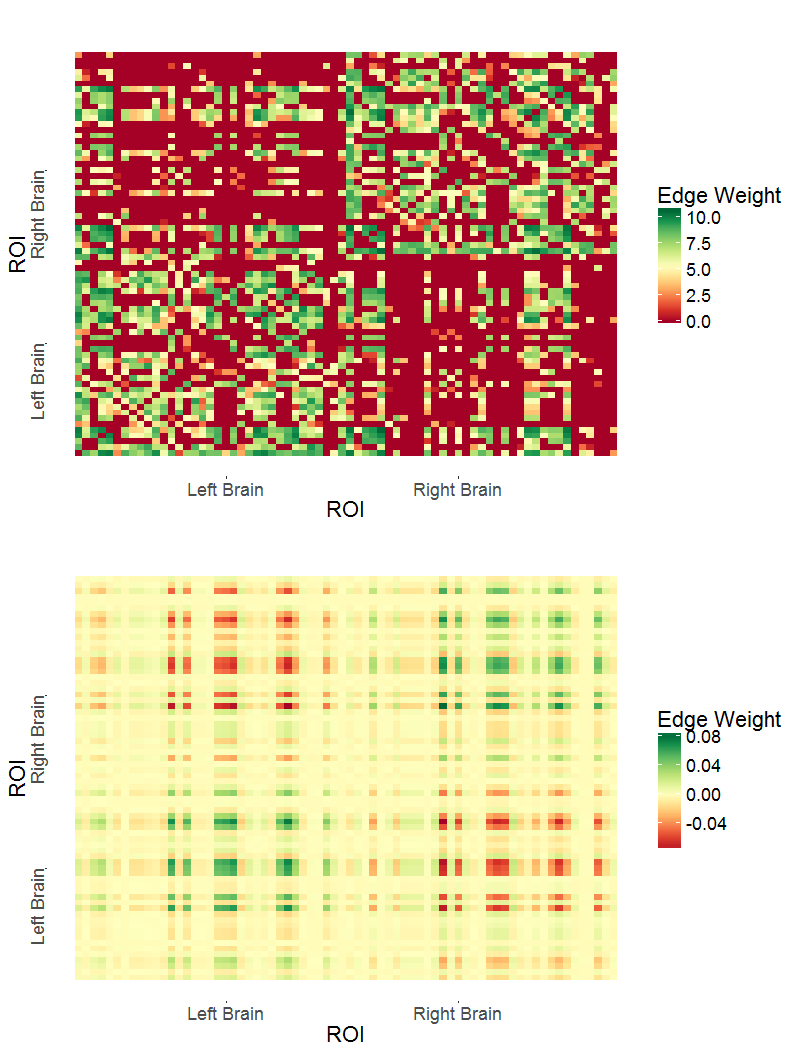
\includegraphics[scale=0.25]{../../figs/cci_data.png}
%\caption{The top panel shows the graph derived from a typical subject. There is much more neural connectivity within each hemisphere. The bottom panel shows the rank one matrix $\hat{h}_6^T\hat{h}_6$, which has positive  connectivity within each hemisphere, but negative  connectivity across hemispheres.}
%\label{fig:cci1}
%\end{cframed}
%\end{figure}
%%
%\clearpage
\end{document}
